\documentclass[journal]{IEEEtran}

\usepackage[utf8]{inputenc}
\usepackage[spanish]{babel}
\usepackage{amsmath}
\usepackage{graphicx}
\usepackage[hyphens]{url}
\usepackage{cite}
\usepackage{hyperref}
\usepackage{booktabs}

\title{Priorizaci\'on Abierta del Riesgo en Presas de M\'exico ante el Vac\'io de Inspecci\'on de CONAGUA}

\author{Manuel Bautista Mej\'ia\thanks{Correo electr\'onico: 18102328bmm@gmail.com}}

\begin{document}

\maketitle

\begin{abstract}
La Comisi\'on Nacional del Agua (CONAGUA) reconoce p\'ublicamente que desconoce el estado f\'isico de cerca de 1{,}000 de sus presas registradas por falta de presupuesto para inspeccionarlas, de un inventario de 836 presas grandes, 4{,}330 chicas, y un estimado de 8{,}000 bordos ni siquiera registrados; 95 presas ya est\'an clasificadas como de alto riesgo \cite{infobae2020presas, eluniversal2021presas}. Este trabajo propone una herramienta de \emph{triage}: un \'indice de prioridad de revisi\'on construido enteramente con datos abiertos de terceros --peligro s\'ismico, lluvia extrema hist\'orica y poblaci\'on cercana-- que no reemplaza la inspecci\'on f\'isica, sino que ordena qu\'e presas sin inspecci\'on reciente ameritan revisi\'on m\'as urgente, haciendo m\'as eficiente el presupuesto de inspecci\'on que la propia CONAGUA admite no tener. El m\'etodo se aplic\'o a las 210 presas que CONAGUA monitorea activamente a trav\'es de su Sistema de Informaci\'on Hidrol\'ogico --el subconjunto p\'ublico disponible, que es precisamente el mejor vigilado y no las 1{,}000 sin supervisi\'on que motivan este trabajo--, combinando la aceleraci\'on m\'axima del terreno (PGA, GEM Foundation), la lluvia de dise\~no a 100 a\~nos ajustada por distribuci\'on Gumbel sobre 33 a\~nos de precipitaci\'on diaria (NASA POWER), y la poblaci\'on en un radio de 30 km (GeoNames) en un \'indice compuesto por percentiles. Los tres factores resultaron pr\'acticamente independientes entre s\'i (correlaciones de Pearson entre 0.09 y 0.29), confirmando que capturan dimensiones de riesgo distintas y no informaci\'on redundante; el resultado no reproduce un ranking dominado por un solo eje geogr\'afico, sino que combina presas de la zona de subducci\'on del Pac\'ifico (Chiapas, Michoac\'an, Guerrero, Oaxaca) con presas de baja sismicidad pero alta densidad poblacional cercana (frontera de Baja California, Puebla). El sistema completo es reproducible de extremo a extremo con c\'odigo abierto y datos p\'ublicos verificables. El \'indice actual mide \emph{peligro} y \emph{exposici\'on}, pero no la tercera dimensi\'on cl\'asica del riesgo --\emph{vulnerabilidad} estructural (altura de cortina, antig\"uedad, estado f\'isico, capacidad del vertedor)-- porque esos campos no est\'an en el cat\'alogo p\'ublico disponible; se solicitaron por separado a trav\'es de la Plataforma Nacional de Transparencia, y su incorporaci\'on al mismo pipeline queda planteada como el paso inmediato hacia un screening estructural completo.
\end{abstract}

\begin{IEEEkeywords}
seguridad de presas, gesti\'on de riesgo, datos abiertos, peligro s\'ismico, transparencia gubernamental, seguridad h\'idrica
\end{IEEEkeywords}

\section{Introducci\'on}
\label{sec:introduccion}

M\'exico tiene registradas 836 presas grandes y 4{,}330 presas peque\~nas, adem\'as de un estimado de 8{,}000 bordos que ni siquiera est\'an registrados \cite{infobae2020presas}. El 76\% del agua del pa\'is se destina a uso agr\'icola, buena parte de ella almacenada o derivada por esta infraestructura \cite{conagua2018estadisticas}. La Comisi\'on Nacional del Agua (CONAGUA) es responsable de vigilar la seguridad de esa red a trav\'es de su Sistema de Seguridad de Presas, pero la propia dependencia ha reconocido p\'ublicamente que desconoce el estado f\'isico y operativo de cerca de 1{,}000 presas por falta de presupuesto y personal para inspeccionarlas, incumpliendo con ello la recomendaci\'on de la Comisi\'on Internacional de Grandes Presas (ICOLD) de inspeccionar la red registrada al menos cada cinco a\~nos \cite{infobae2020presas, eluniversal2021presas}. De las presas s\'i evaluadas, 95 est\'an clasificadas actualmente como de alto riesgo \cite{infobae2020presas}. CONAGUA reconoce adem\'as que el riesgo de falla es ``permanente'', dado que la variabilidad hidrol\'ogica anual se ha vuelto m\'as abrupta por el cambio clim\'atico, adem\'as de fallas mec\'anicas, vandalismo y ausencia de mantenimiento \cite{infobae2020presas}.

Esta brecha no es un problema abstracto: buena parte de las presas peque\~nas y bordos sostienen el riego de comunidades agr\'icolas enteras, y muchas de las presas grandes del pa\'is llevan m\'as de 50 a\~nos en operaci\'on sin haber recibido mantenimiento mayor \cite{tecscience2023infraestructura}. La falla de una presa --por sismo, por una tormenta que excede la capacidad de dise\~no del vertedor, o simplemente por deterioro acumulado-- pone en riesgo directo a las poblaciones aguas abajo. El problema, en el fondo, es de asignaci\'on de un recurso escaso: si CONAGUA no tiene presupuesto para inspeccionar toda la red, la pregunta relevante no es \emph{si} se puede inspeccionar todo, sino \emph{qu\'e} se inspecciona primero.

Ese es exactamente el tipo de pregunta que un sistema de \emph{triage} basado en datos abiertos puede ayudar a responder, sin sustituir en ning\'un momento el criterio de un ingeniero especialista ni la inspecci\'on f\'isica en campo. La literatura en ingenier\'ia s\'ismica ya ofrece metodolog\'ias de evaluaci\'on r\'apida (\emph{screening}) para priorizar portafolios grandes de presas \cite{hariri2018prioritization, natural2023multiscale}, pero est\'an dise\~nadas y demostradas sobre inventarios que ya cuentan con datos estructurales b\'asicos (altura, geometr\'ia, a\~no de construcci\'on) capturados por el propio operador de la presa. Ese no es el caso de M\'exico: los atributos estructurales de la mayor parte del inventario, y en particular de las \(\sim\)1{,}000 presas sin supervisi\'on reciente que motivan este trabajo, no est\'an disponibles p\'ublicamente --viven \'unicamente en el buscador interactivo del Sistema de Seguridad de Presas, sin opci\'on de descarga masiva.

Este trabajo construye y eval\'ua, con ese vac\'io de datos como punto de partida expl\'icito, un \'indice de prioridad de revisi\'on basado \'unicamente en fuentes de datos abiertas y verificables: peligro s\'ismico, lluvia extrema hist\'orica, y poblaci\'on cercana. Se aplica sobre el subconjunto p\'ublico disponible --las 210 presas que CONAGUA monitorea activamente-- como validaci\'on metodol\'ogica, mientras se gestiona por separado, a trav\'es de una solicitud de transparencia gubernamental, el acceso al inventario completo y a los atributos estructurales necesarios para convertir este \'indice de exposici\'on en un screening de riesgo estructural pleno.

La Secci\'on \ref{sec:marco_teorico} revisa la literatura de evaluaci\'on de riesgo en portafolios de presas y ubica el vac\'io de datos mexicano frente a ella. La Secci\'on \ref{sec:metodologia} describe las fuentes de datos y la construcci\'on del \'indice. La Secci\'on \ref{sec:resultados} reporta su aplicaci\'on sobre las 210 presas monitoreadas. La Secci\'on \ref{sec:discusion} interpreta esos resultados y sus limitaciones. La Secci\'on \ref{sec:conclusiones} cierra con el alcance logrado y el trabajo pendiente.

\section{Marco Te\'orico}
\label{sec:marco_teorico}

\subsection{Riesgo como producto de peligro, exposici\'on y vulnerabilidad}

La gesti\'on de riesgo de desastres descompone convencionalmente el riesgo en tres factores multiplicativos: \emph{peligro} (la probabilidad de que ocurra un evento f\'isico detonante, p. ej. un sismo o una tormenta extrema), \emph{exposici\'on} (qu\'e o qui\'en est\'a en la trayectoria de ese evento) y \emph{vulnerabilidad} (qu\'e tan susceptible es el elemento expuesto a sufrir da\~no dado el evento). Aplicado a una presa, el peligro es externo al sitio (sismicidad regional, r\'egimen de lluvias), la exposici\'on es la poblaci\'on y la infraestructura aguas abajo, y la vulnerabilidad es intr\'inseca a la estructura misma --su geometr\'ia, edad, material y estado de conservaci\'on--. Los tres factores son necesarios: una presa en zona de bajo peligro s\'ismico pero estructuralmente deteriorada puede representar m\'as riesgo que una presa robusta en zona de alto peligro.

\subsection{Metodolog\'ias de \emph{screening} para portafolios grandes de presas}

Cuando un operador es responsable de cientos o miles de presas, evaluar cada una con un an\'alisis estructural detallado es inviable en tiempo y presupuesto; de ah\'i que la literatura en ingenier\'ia s\'ismica haya desarrollado metodolog\'ias de evaluaci\'on r\'apida (\emph{screening}) para priorizar qu\'e presas ameritan un an\'alisis m\'as profundo primero. Hariri-Ardebili y Nuss \cite{hariri2018prioritization} proponen un \'indice sem\'i-cuantitativo de priorizaci\'on s\'ismica que combina par\'ametros de la presa, del embalse, y de riesgo aguas abajo. Un enfoque m\'as reciente, orientado a fases de preparaci\'on y respuesta a emergencias, propone una herramienta multiescala que arranca con an\'alisis simplificados de cuerpo r\'igido en dos dimensiones y solo escala a modelos no lineales cuando el screening inicial lo justifica, precisamente para mantener el proceso \'agil y econ\'omico sobre portafolios grandes \cite{natural2023multiscale}. Ambos enfoques, sin embargo, presuponen que el operador ya cuenta con los atributos b\'asicos de cada presa del portafolio --altura, geometr\'ia, tipo de cortina-- capturados en un inventario propio; el problema que resuelven es c\'omo \emph{ordenar} un an\'alisis m\'as profundo, no c\'omo operar cuando esos atributos b\'asicos no est\'an disponibles en absoluto para la mayor parte del portafolio.

\subsection{El vac\'io de datos como el problema previo a resolver en M\'exico}

Ese es precisamente el punto en el que la situaci\'on de M\'exico se aparta de los casos de estudio t\'ipicos en la literatura. No se trata de decidir qu\'e nivel de an\'alisis estructural aplicar --pseudo-est\'atico, din\'amico lineal, no lineal-- sino de que los datos de entrada m\'as b\'asicos para \emph{cualquiera} de esos niveles (altura de cortina, a\~no de construcci\'on, capacidad del vertedor, estado f\'isico y fecha de \'ultima inspecci\'on) no est\'an publicados para la mayor parte de las presas del pa\'is, y en particular no lo est\'an para el subconjunto de \(\sim\)1{,}000 presas que CONAGUA reconoce no haber inspeccionado recientemente \cite{infobae2020presas} --el subconjunto donde un \'indice de priorizaci\'on ser\'ia m\'as \'util--. Esta situaci\'on no es exclusiva de M\'exico: la literatura reconoce que los vac\'ios de datos espaciales para presas peque\~nas y medianas persisten en regiones en desarrollo, con omisiones y actualizaciones retrasadas que dificultan estimar el riesgo de desastre asociado a esta infraestructura \cite{natural2023multiscale}.

\subsection{Contribuci\'on de este trabajo}

Frente a ese vac\'io, este trabajo no intenta emular un an\'alisis estructural que los datos disponibles no permiten. En su lugar, construye la mitad del problema de riesgo que s\'i es calculable enteramente con datos abiertos de terceros --peligro s\'ismico regional, r\'egimen de lluvia extrema, y exposici\'on poblacional-- como un \'indice de \emph{priorizaci\'on de inspecci\'on}, dejando expl\'icito qu\'e falta (la vulnerabilidad estructural) y d\'onde se est\'a gestionando (una solicitud de transparencia gubernamental, detallada en la Secci\'on \ref{sec:metodologia}). Esto sigue el esp\'iritu del \emph{screening} en dos etapas de \cite{natural2023multiscale} --evaluaci\'on r\'apida primero, an\'alisis detallado despu\'es solo donde se justifique-- pero aplicado a la etapa previa que la literatura revisada no aborda expl\'icitamente: qu\'e hacer cuando ni siquiera el inventario b\'asico es p\'ublico.

\section{Metodolog\'ia}
\label{sec:metodologia}

\subsection{\'Area de estudio y cat\'alogo de presas}

El cat\'alogo base proviene del Sistema de Informaci\'on Hidrol\'ogica de CONAGUA \cite{sih2026catalogo}, que publica nombre, clave, ubicaci\'on (latitud/longitud), municipio, estado y cuenca de disponibilidad de 210 presas con estaci\'on de monitoreo activa, distribuidas en 26 estados. Este es un subconjunto p\'ublico y descargable del inventario nacional, pero corresponde precisamente a las presas \textbf{mejor} vigiladas por CONAGUA --no al subconjunto de \(\sim\)1{,}000 presas sin inspecci\'on reciente que motiva este trabajo (Secci\'on \ref{sec:introduccion})--. El sitio que administra el inventario completo, incluyendo atributos estructurales (altura de cortina, capacidad del vertedor, a\~no de construcci\'on, estado f\'isico y operativo) est\'a protegido contra descarga autom\'atizada por un firewall comercial contra bots; esos campos se solicitaron por separado a trav\'es de la Plataforma Nacional de Transparencia de M\'exico, con respuesta legal esperada en un plazo de 20 a 30 d\'ias h\'abiles. Este art\'iculo reporta la metodolog\'ia y su validaci\'on sobre el subconjunto de 210 presas disponible hoy; el c\'odigo (Secci\'on \ref{sec:conclusiones}) est\'a preparado para incorporar el inventario completo y los atributos estructurales en cuanto est\'en disponibles.

\subsection{Peligro s\'ismico}
\label{sec:metodologia_sismico}

El peligro s\'ismico de cada presa se obtuvo del \emph{Global Seismic Hazard Map} (versi\'on 2023.1) de la Global Earthquake Model (GEM) Foundation \cite{gem2023hazard}, un raster global de aceleraci\'on m\'axima del terreno (PGA, en fracci\'on de $g$) con 10\% de probabilidad de excedencia en 50 a\~nos (periodo de retorno \(\approx\)475 a\~nos), calculado para condiciones de roca de referencia (\(V_{s30}\) de 760--800 m/s) a una resoluci\'on de 3 arcominutos (\(\approx\)6 km). Por tratarse de condiciones de roca de referencia, el valor no incluye amplificaci\'on por sitio (p. ej. suelos blandos como los de buena parte de la Ciudad de M\'exico); es una base razonable para un \emph{screening}, no un estudio de sitio espec\'ifico. El PGA de cada presa se extrajo por muestreo directo del raster en sus coordenadas (latitud, longitud).

\subsection{Lluvia extrema hist\'orica}
\label{sec:metodologia_lluvia}

Para cada presa se descarg\'o la serie diaria de precipitaci\'on corregida (\texttt{PRECTOTCORR}) de NASA POWER \cite{nasapower2026} para el periodo 1991--2023 (33 a\~nos) en sus coordenadas exactas. De cada serie se extrajo el m\'aximo anual de precipitaci\'on diaria, y a esos m\'aximos anuales se ajust\'o una distribuci\'on de valores extremos tipo I (Gumbel), el m\'etodo est\'andar en hidrolog\'ia para estimar la magnitud de eventos de lluvia extrema a partir de series hist\'oricas \cite{chow1988applied}. De la distribuci\'on ajustada se estim\'o la lluvia de dise\~no correspondiente a un periodo de retorno de 100 a\~nos, como indicador de qu\'e tan severo es el r\'egimen de lluvia extrema en la ubicaci\'on de cada presa.

\subsection{Poblaci\'on cercana}
\label{sec:metodologia_poblacion}

Como proxy de exposici\'on --qu\'e tan grave ser\'ia una falla-- se calcul\'o la poblaci\'on total dentro de un radio de 30 km de cada presa, sumando la poblaci\'on reportada de todas las localidades pobladas (c\'odigo de \emph{feature class} \texttt{P} en la nomenclatura de GeoNames) de M\'exico con poblaci\'on conocida, seg\'un el volcado p\'ublico de GeoNames \cite{geonames2026}. La distancia se calcul\'o con la f\'ormula de haversine sobre las coordenadas de cada presa y cada localidad. Este es expl\'icitamente un proxy en l\'inea recta, no una zona de inundaci\'on real: estimar la mancha de inundaci\'on efectiva aguas abajo de una falla requerir\'ia un modelo de elevaci\'on digital y an\'alisis hidrol\'ogico de flujo, fuera del alcance de este trabajo (Secci\'on \ref{sec:discusion}).

\subsection{\'Indice compuesto de prioridad}
\label{sec:metodologia_indice}

Los tres factores --PGA, lluvia de dise\~no a 100 a\~nos, y poblaci\'on en 30 km-- tienen unidades y distribuciones muy distintas (las tres est\'an fuertemente sesgadas a la derecha, con pocas presas de valores muy altos). Por eso cada uno se convirti\'o a un percentil (0--100) dentro del conjunto de 210 presas, en vez de normalizar por media y desviaci\'on est\'andar: el percentil es robusto a esa asimetr\'ia y directamente interpretable (``esta presa est\'a en el percentil 90 de peligro s\'ismico del pa\'is''). El percentil s\'ismico y el hidrol\'ogico --ambos factores de \emph{peligro}-- se promediaron primero entre s\'i, y ese promedio se combin\'o en partes iguales con el percentil de poblaci\'on --el factor de \emph{exposici\'on}--, de modo que ning\'un factor domine el \'indice final solo por tener dos entradas en vez de una:

\begin{equation}
I = \frac{1}{2}\left(\frac{P_{\text{s\'ismico}} + P_{\text{hidrol\'ogico}}}{2}\right) + \frac{1}{2} P_{\text{poblacional}}
\label{eq:indice}
\end{equation}

donde \(P_x\) denota el percentil del factor \(x\). El resultado, $I \in [0, 100]$, es el \'indice de prioridad de revisi\'on reportado en la Secci\'on \ref{sec:resultados}.

\subsection{Reproducibilidad}

Todo el pipeline --descarga y cacheo de datos, c\'alculo de los tres factores, construcci\'on del \'indice y generaci\'on del mapa-- est\'a implementado en Python y disponible como c\'odigo abierto (Secci\'on \ref{sec:conclusiones}). Las fuentes de datos son p\'ublicas y no requieren llave de acceso, con la excepci\'on del cat\'alogo base de CONAGUA (Secci\'on \ref{sec:metodologia}), que se descarg\'o manualmente por el firewall anti-bots del sitio de origen y se conserva como archivo est\'atico en el repositorio.

\section{Resultados}
\label{sec:resultados}

\subsection{Distribuci\'on de los factores}

Sobre las 210 presas del cat\'alogo, el PGA vari\'o entre 0.0085$g$ y 0.735$g$ (mediana 0.104$g$), la lluvia de dise\~no a 100 a\~nos entre 40.4 mm y 211.2 mm/d\'ia (mediana 60.2 mm/d\'ia), y la poblaci\'on en 30 km entre 456 y 28.4 millones de habitantes (mediana 198{,}658), esta \'ultima con una asimetr\'ia much\'isimo mayor que los otros dos factores --consistente con que la poblaci\'on se concentra en un n\'umero peque\~no de zonas metropolitanas grandes--.

\subsection{Independencia entre factores}

La correlaci\'on de Pearson entre los percentiles de los tres factores fue baja: 0.086 entre el s\'ismico y el hidrol\'ogico, 0.290 entre el s\'ismico y el poblacional, y $-0.301$ entre el hidrol\'ogico y el poblacional. Esta independencia relativa es deseable: confirma que los tres factores capturan dimensiones de riesgo distintas y que el \'indice compuesto (Ecuaci\'on \ref{eq:indice}) no est\'a dominado impl\'icitamente por una sola de ellas.

\subsection{Ranking de prioridad}

La Tabla \ref{tab:top10} reporta las diez presas con mayor \'indice de prioridad. El resultado no reproduce un ranking dominado por un solo criterio geogr\'afico: combina presas de la zona de subducci\'on de la costa del Pac\'ifico y el sureste --Manuel Moreno Torres (Chiapas), La Cangrejera (Veracruz), Jos\'e Mar\'ia Morelos y Pav\'on (Michoac\'an)--, cuyo peso proviene principalmente del peligro s\'ismico e hidrol\'ogico, con presas de sismicidad moderada pero muy alta densidad poblacional cercana --El Carrizo y Abelardo L. Rodr\'iguez, ambas en la zona metropolitana de Tijuana, Baja California; Manuel \'Avila Camacho, cerca de la zona metropolitana de Puebla--.

\begin{table}[htbp]
\centering
\caption{Top 10 presas por \'indice de prioridad de revisi\'on}
\label{tab:top10}
\begin{tabular}{@{}llr@{}}
\toprule
Clave & Estado & \'Indice \\
\midrule
CHICP & Chiapas & 88.3 \\
LCAVC & Veracruz & 87.6 \\
CRRBN & Baja California & 82.1 \\
SOLPB & Puebla & 82.0 \\
BDDPB & Puebla & 81.8 \\
ALRBN & Baja California & 81.6 \\
VILMC & Michoac\'an & 81.5 \\
SNLSI & Sinaloa & 80.1 \\
ELZBN & Baja California & 77.9 \\
COIMC & Michoac\'an & 77.6 \\
\bottomrule
\end{tabular}
\end{table}

La Figura \ref{fig:mapa} muestra el \'indice de prioridad geogr\'aficamente. Las presas de menor prioridad se concentran en el altiplano central --zona de baja sismicidad y lluvia moderada--, mientras que las de mayor prioridad se distribuyen en la periferia del pa\'is: la costa del Pac\'ifico y el sureste por peligro combinado, y los n\'ucleos urbanos grandes (frontera norte, Puebla) por exposici\'on poblacional.

\begin{figure}[htbp]
\centering
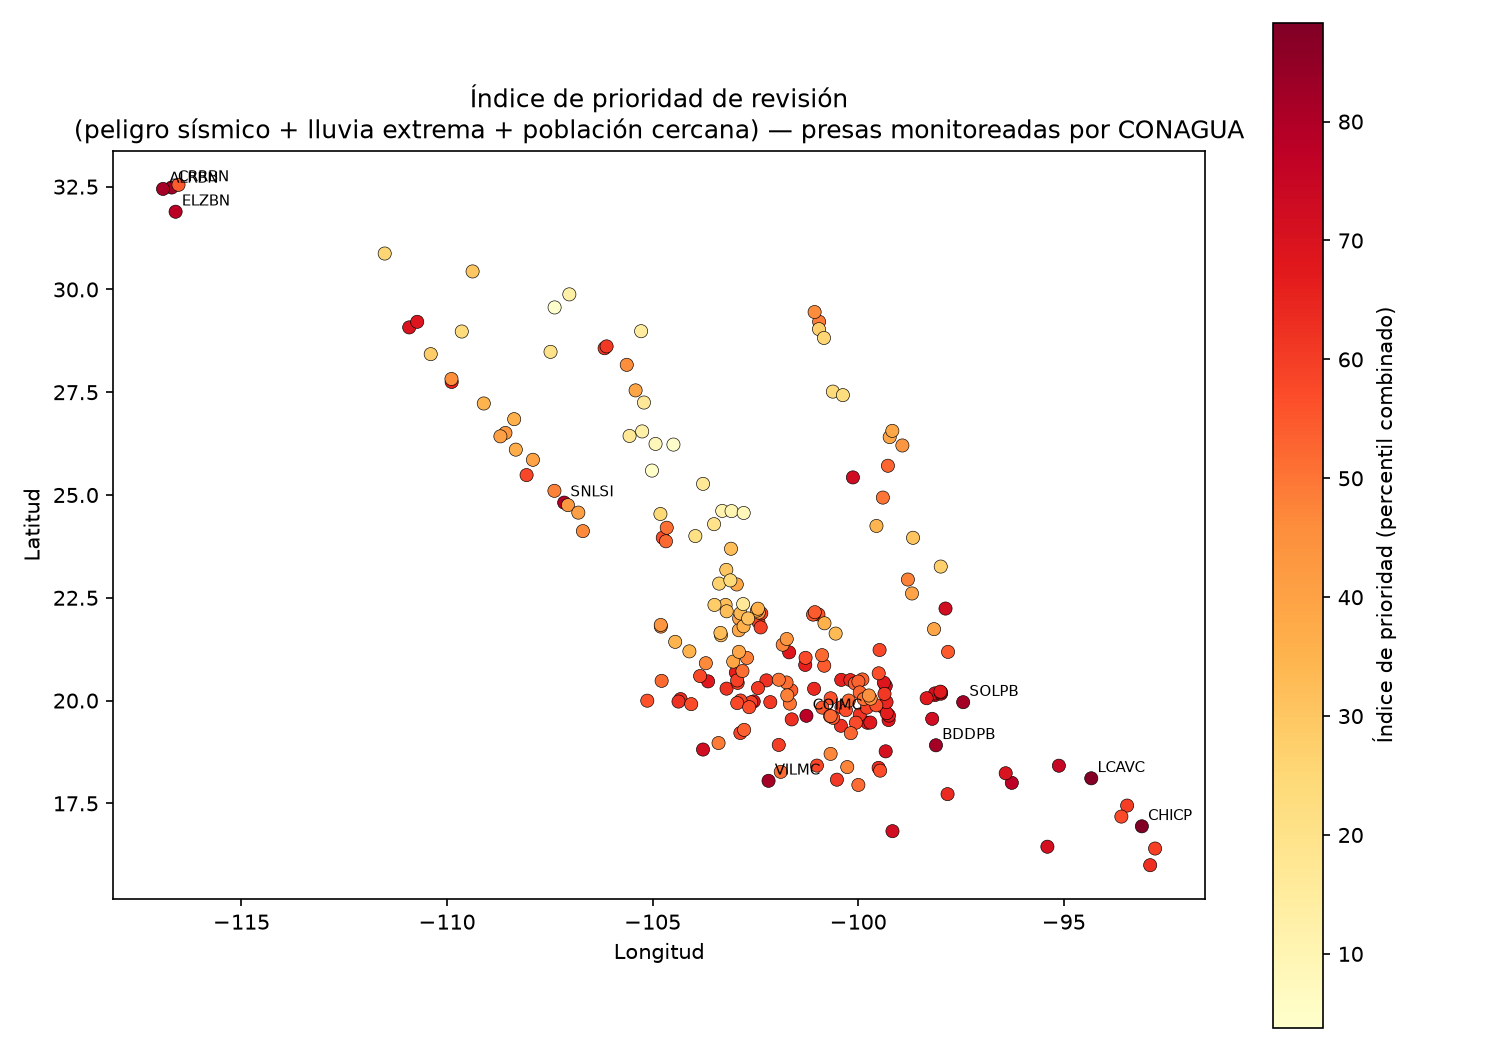
\includegraphics[width=\columnwidth]{figures/mapa_prioridad_presas.png}
\caption{\'Indice de prioridad de revisi\'on por presa (peligro s\'ismico + lluvia extrema + poblaci\'on cercana), 210 presas monitoreadas por CONAGUA.}
\label{fig:mapa}
\end{figure}

\section{Discusi\'on}
\label{sec:discusion}

\subsection{Lo que el \'indice s\'i mide}

El patr\'on geogr\'afico del \'indice (Figura \ref{fig:mapa}) es consistente con la sismolog\'ia y la hidrolog\'ia conocidas de M\'exico: las presas de mayor peligro s\'ismico se concentran en la zona de subducci\'on de la placa de Cocos a lo largo de la costa del Pac\'ifico (Chiapas, Oaxaca, Guerrero, Michoac\'an, Colima), mientras que el altiplano central --geol\'ogicamente m\'as estable-- domina el extremo de baja prioridad. La aparici\'on de presas de la frontera de Baja California y de la zona metropolitana de Puebla en el top 10 --pese a su sismicidad moderada-- ilustra precisamente el valor de combinar peligro con exposici\'on: son presas donde el evento detonante es menos probable, pero donde una falla afectar\'ia a una poblaci\'on much\'isimo mayor. Ninguno de los dos factores por separado habr\'ia identificado ese patr\'on.

\subsection{Lo que el \'indice todav\'ia no mide}

Este trabajo mide \emph{peligro} y \emph{exposici\'on}, pero no \emph{vulnerabilidad} --la tercera dimensi\'on cl\'asica del riesgo (Secci\'on \ref{sec:marco_teorico})--. Una presa puede tener baja prioridad en este \'indice por estar en una zona de peligro moderado y baja densidad poblacional cercana, y a\'un as\'i representar un riesgo alto si su estructura est\'a severamente deteriorada. Ese dato --altura de cortina, a\~no de construcci\'on, capacidad del vertedor, estado f\'isico y fecha de \'ultima inspecci\'on-- es precisamente el que CONAGUA no publica para la mayor parte del inventario (Secci\'on \ref{sec:introduccion}), y el que se solicit\'o por separado v\'ia transparencia gubernamental. Hasta que esa informaci\'on est\'e disponible, este \'indice debe leerse como una priorizaci\'on de \emph{d\'onde mirar primero}, no como un diagn\'ostico de seguridad estructural.

Una segunda limitaci\'on es de escala: el an\'alisis cubre las 210 presas que CONAGUA ya monitorea activamente, que son estructuralmente las mejor vigiladas del pa\'is --no las \(\sim\)1{,}000 sin inspecci\'on reciente que motivan este trabajo (Secci\'on \ref{sec:introduccion})--, ni los \(\sim\)8{,}000 bordos no registrados. El valor de este resultado es metodol\'ogico: demuestra que el \'indice es calculable y produce un ranking geogr\'aficamente coherente sobre un subconjunto verificable, listo para aplicarse al inventario completo en cuanto est\'e disponible.

Una tercera limitaci\'on es de precisi\'on de cada factor individual. El PGA se calcula para condiciones de roca de referencia y no incorpora amplificaci\'on por sitio (Secci\'on \ref{sec:metodologia_sismico}); la poblaci\'on cercana es un radio en l\'inea recta, no una zona de inundaci\'on real trazada por un modelo de elevaci\'on digital (Secci\'on \ref{sec:metodologia_poblacion}); y la lluvia de dise\~no asume que la distribuci\'on Gumbel ajustada sobre 33 a\~nos de registro es representativa del r\'egimen extremo de cada sitio, sin correcci\'on por tendencias de cambio clim\'atico. Cada una de estas simplificaciones es razonable para un \emph{screening} de primera pasada, pero ninguna sustituye un estudio de sitio o un modelo hidrol\'ogico de detalle para una presa espec\'ifica que el \'indice se\~nale como prioritaria.

\subsection{Sobre la dependencia de una solicitud de transparencia}

Que el paso metodol\'ogico m\'as importante pendiente de este trabajo --incorporar vulnerabilidad estructural real-- dependa de una solicitud de acceso a informaci\'on p\'ublica, y no de una limitaci\'on t\'ecnica, es en s\'i mismo un hallazgo relevante: refuerza emp\'iricamente el reclamo de CONAGUA de que el vac\'io de supervisi\'on de presas peque\~nas es, ante todo, un problema de recursos y de transparencia, no de falta de metodolog\'ias disponibles para atenderlo.

\section{Conclusiones}
\label{sec:conclusiones}

Este trabajo construy\'o un \'indice de prioridad de revisi\'on para presas mexicanas, enteramente a partir de datos abiertos de terceros --peligro s\'ismico (GEM Foundation), lluvia extrema hist\'orica (NASA POWER) y poblaci\'on cercana (GeoNames)-- motivado por el reconocimiento p\'ublico de CONAGUA de que carece de presupuesto para inspeccionar cerca de 1{,}000 de sus presas registradas. Aplicado a las 210 presas que CONAGUA s\'i monitorea activamente, el \'indice produjo un ranking geogr\'aficamente coherente con la sismolog\'ia e hidrolog\'ia conocidas del pa\'is, combinando de forma no trivial presas de alto peligro f\'isico con presas de alta exposici\'on poblacional --tres factores que result\'aron pr\'acticamente independientes entre s\'i (Secci\'on \ref{sec:resultados})--, demostrando que la metodolog\'ia es t\'ecnicamente viable y reproducible con recursos de un solo investigador y sin financiamiento institucional.

El trabajo es expl\'icito, sin embargo, en que mide \emph{peligro y exposici\'on}, no \emph{vulnerabilidad estructural} --y en que se aplic\'o sobre el subconjunto de presas mejor vigilado del pa\'is, no sobre las que motivan el proyecto--. Cerrar esa brecha depende de una solicitud de acceso a informaci\'on p\'ublica presentada ante la Plataforma Nacional de Transparencia, pidiendo el inventario nacional completo con atributos estructurales (altura de cortina, capacidad del vertedor, a\~no de construcci\'on, estado f\'isico y fecha de \'ultima inspecci\'on). El pipeline de este trabajo --disponible como c\'odigo abierto en \url{https://github.com/mxnueel/riesgo-presas-mexico}-- est\'a preparado para incorporar esos datos en cuanto se reciban, extendiendo el an\'alisis del subconjunto de 210 presas monitoreadas al inventario completo de \(\sim\)5{,}166 presas registradas y, en la medida en que se documenten, a los \(\sim\)8{,}000 bordos no registrados.

Como trabajo futuro inmediato, adem\'as de incorporar la vulnerabilidad estructural real, quedan pendientes: reemplazar el proxy de poblaci\'on en l\'inea recta por una zona de inundaci\'on real derivada de un modelo de elevaci\'on digital; e incorporar la clasificaci\'on de riesgo ya publicada por CONAGUA para las 95 presas de alto riesgo conocidas, como una verificaci\'on directa de si el \'indice las se\~nala consistentemente como prioritarias.


\bibliographystyle{IEEEtran}
\bibliography{referencias}

\end{document}
